%!TeX encoding = UTF-8
%!TeX program = xelatex
\documentclass[notheorems, aspectratio=54]{beamer}
% aspectratio: 1610, 149, 54, 43(default), 32

\usepackage{latexsym}
\usepackage{amsmath,amssymb}
\usepackage{mathtools}
\usepackage{color,xcolor}
\usepackage{graphicx}
\usepackage{algorithm}
\usepackage{amsthm}
\usepackage{lmodern} % 解决 font warning
% \usepackage[UTF8]{ctex}
\usepackage{animate} % insert gif

\usepackage{lipsum} % To generate test text 
\usepackage{ulem} % 下划线,波浪线

\usepackage{listings} % display code on slides; don't forget [fragile] option after \begin{frame}

% ----------------------------------------------
% tikx
\usepackage{framed}
\usepackage{tikz}
\usepackage{pgf}
\usetikzlibrary{calc,trees,positioning,arrows,chains,shapes.geometric,%
	decorations.pathreplacing,decorations.pathmorphing,shapes,%
	matrix,shapes.symbols}
\pgfmathsetseed{1} % To have predictable results
% Define a background layer, in which the parchment shape is drawn
\pgfdeclarelayer{background}
\pgfsetlayers{background,main}

% define styles for the normal border and the torn border
\tikzset{
	normal border/.style={orange!30!black!10, decorate, 
		decoration={random steps, segment length=2.5cm, amplitude=.7mm}},
	torn border/.style={orange!30!black!5, decorate, 
		decoration={random steps, segment length=.5cm, amplitude=1.7mm}}}

% Macro to draw the shape behind the text, when it fits completly in the
% page
\def\parchmentframe#1{
	\tikz{
		\node[inner sep=2em] (A) {#1};  % Draw the text of the node
		\begin{pgfonlayer}{background}  % Draw the shape behind
			\fill[normal border] 
			(A.south east) -- (A.south west) -- 
			(A.north west) -- (A.north east) -- cycle;
\end{pgfonlayer}}}

% Macro to draw the shape, when the text will continue in next page
\def\parchmentframetop#1{
	\tikz{
		\node[inner sep=2em] (A) {#1};    % Draw the text of the node
		\begin{pgfonlayer}{background}    
			\fill[normal border]              % Draw the ``complete shape'' behind
			(A.south east) -- (A.south west) -- 
			(A.north west) -- (A.north east) -- cycle;
			\fill[torn border]                % Add the torn lower border
			($(A.south east)-(0,.2)$) -- ($(A.south west)-(0,.2)$) -- 
			($(A.south west)+(0,.2)$) -- ($(A.south east)+(0,.2)$) -- cycle;
\end{pgfonlayer}}}

% Macro to draw the shape, when the text continues from previous page
\def\parchmentframebottom#1{
	\tikz{
		\node[inner sep=2em] (A) {#1};   % Draw the text of the node
		\begin{pgfonlayer}{background}   
			\fill[normal border]             % Draw the ``complete shape'' behind
			(A.south east) -- (A.south west) -- 
			(A.north west) -- (A.north east) -- cycle;
			\fill[torn border]               % Add the torn upper border
			($(A.north east)-(0,.2)$) -- ($(A.north west)-(0,.2)$) -- 
			($(A.north west)+(0,.2)$) -- ($(A.north east)+(0,.2)$) -- cycle;
\end{pgfonlayer}}}

% Macro to draw the shape, when both the text continues from previous page
% and it will continue in next page
\def\parchmentframemiddle#1{
	\tikz{
		\node[inner sep=2em] (A) {#1};   % Draw the text of the node
		\begin{pgfonlayer}{background}   
			\fill[normal border]             % Draw the ``complete shape'' behind
			(A.south east) -- (A.south west) -- 
			(A.north west) -- (A.north east) -- cycle;
			\fill[torn border]               % Add the torn lower border
			($(A.south east)-(0,.2)$) -- ($(A.south west)-(0,.2)$) -- 
			($(A.south west)+(0,.2)$) -- ($(A.south east)+(0,.2)$) -- cycle;
			\fill[torn border]               % Add the torn upper border
			($(A.north east)-(0,.2)$) -- ($(A.north west)-(0,.2)$) -- 
			($(A.north west)+(0,.2)$) -- ($(A.north east)+(0,.2)$) -- cycle;
\end{pgfonlayer}}}

% Define the environment which puts the frame
% In this case, the environment also accepts an argument with an optional
% title (which defaults to ``Example'', which is typeset in a box overlaid
% on the top border
\newenvironment{parchment}[1][Example]{%
	\def\FrameCommand{\parchmentframe}%
	\def\FirstFrameCommand{\parchmentframetop}%
	\def\LastFrameCommand{\parchmentframebottom}%
	\def\MidFrameCommand{\parchmentframemiddle}%
	\vskip\baselineskip
	\MakeFramed {\FrameRestore}
	\noindent\tikz\node[inner sep=1ex, draw=black!20,fill=white, 
	anchor=west, overlay] at (0em, 2em) {\sffamily#1};\par}%
{\endMakeFramed}

% ----------------------------------------------

\mode<presentation>{
	\usetheme{CambridgeUS}
	% Boadilla CambridgeUS
	% default Antibes Berlin Copenhagen
	% Madrid Montpelier Ilmenau Malmoe
	% Berkeley Singapore Warsaw
	\usecolortheme{beaver}
	% beetle, beaver, orchid, whale, dolphin
	\useoutertheme{infolines}
	% infolines miniframes shadow sidebar smoothbars smoothtree split tree
	\useinnertheme{circles}
	% circles, rectanges, rounded, inmargin
}
% 设置 block 颜色
\setbeamercolor{block title}{bg=red!30,fg=white}

\newcommand{\reditem}[1]{\setbeamercolor{item}{fg=red}\item #1}

% 缩放公式大小
\newcommand*{\Scale}[2][4]{\scalebox{#1}{\ensuremath{#2}}}

% 解决 font warning
\renewcommand\textbullet{\ensuremath{\bullet}}

% ---------------------------------------------------------------------
% flow chart
\tikzset{
	>=stealth',
	punktchain/.style={
		rectangle, 
		rounded corners, 
		% fill=black!10,
		draw=white, very thick,
		text width=6em,
		minimum height=2em, 
		text centered, 
		on chain
	},
	largepunktchain/.style={
		rectangle,
		rounded corners,
		draw=white, very thick,
		text width=10em,
		minimum height=2em,
		on chain
	},
	line/.style={draw, thick, <-},
	element/.style={
		tape,
		top color=white,
		bottom color=blue!50!black!60!,
		minimum width=6em,
		draw=blue!40!black!90, very thick,
		text width=6em, 
		minimum height=2em, 
		text centered, 
		on chain
	},
	every join/.style={->, thick,shorten >=1pt},
	decoration={brace},
	tuborg/.style={decorate},
	tubnode/.style={midway, right=2pt},
	font={\fontsize{10pt}{12}\selectfont},
}
% ---------------------------------------------------------------------

% code setting
\lstset{
	language=C++,
	basicstyle=\ttfamily\footnotesize,
	keywordstyle=\color{red},
	breaklines=true,
	xleftmargin=2em,
	numbers=left,
	numberstyle=\color[RGB]{222,155,81},
	frame=leftline,
	tabsize=4,
	breakatwhitespace=false,
	showspaces=false,               
	showstringspaces=false,
	showtabs=false,
	morekeywords={Str, Num, List},
}


% ---------------------------------------------------------------------

%% preamble
\title[A brief intro to GCNs]{A brief introduction to \\ Graph Convolutional Networks}
% \subtitle{The subtitle}
\author{Nhut-Nam Le}
\institute[HCMUS]{Computer Science Department, Information Technology, HCMUS, VNU}

% -------------------------------------------------------------

\begin{document}
	
	%% title frame
	\begin{frame}
		\titlepage
	\end{frame}
	
	%% normal frame
	\begin{frame}{Table of contents}
		\tableofcontents
	\end{frame}
	\section{The motivation}
	\begin{frame}{The motivation}
		\begin{itemize}
			\item Convolutional Neural Network which can only operate on regular Euclidean data like images (2D grid) and text (sequences).
			\item Network Embedding achieved breakthoughs like Word Embeddings, DeepWalk, node2vec, LINE, TADW. However, they still suffer from two drawbacks:
			\begin{itemize}
				\item No parameters are shared between nodes in the encoder
				\item The direct embedding methods lack the ability of generalization
			\end{itemize}
		\end{itemize}
	\end{frame}
	\section{Convolutional Neural Networks}
	\begin{frame}{From Image with Convolutional Networks}
		Convolution operator in Digital Image Processing
		\begin{equation}
			\text{Output}(x, y) = (K * \text{Input})(x, y) = \sum_m\sum_n\text{Input}(x-m, y-m)K(m,n)
		\end{equation}
		Cross-correlation in CNN
		\begin{equation}
			\text{Output}(x, y) = (K * \text{Input})(x, y) = \sum_m\sum_n\text{Input}(x+m, y+m)K(m,n)
		\end{equation}
		\begin{figure}[H]
			\centering
			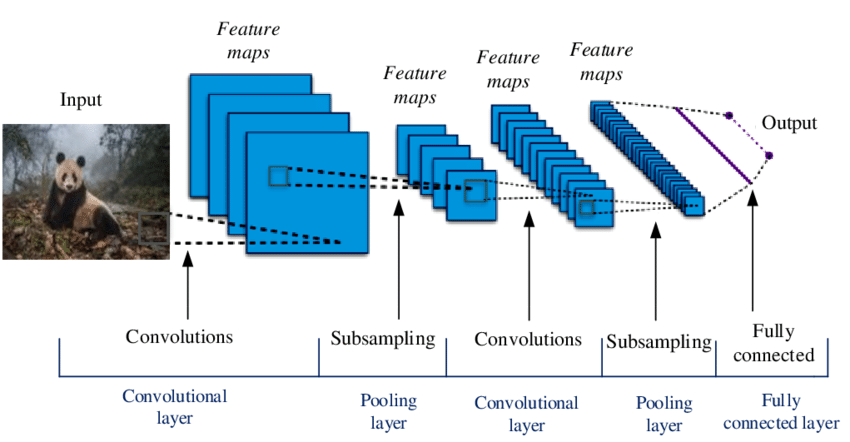
\includegraphics[width=.75\linewidth]{figs/An-example-of-a-simple-CNN-architecture.png}
			\label{fig:writing-thesis}
		\end{figure}
	\end{frame}
	\section{Graph Convolutional Networks}
	\begin{frame}{Overview}
		We can categorize as
		\begin{itemize}
			\item Spectral approaches work with a spectral representation of the graphs, the learned filters depend on the Laplacian eigenbasis, which depends on the graph structure \cite{intrognn2020}
			\item Spatial approaches defines convolutions directly on the graph, operating on spatially close neighbors \cite{intrognn2020}
		\end{itemize}
		\begin{figure}[H]
			\centering
			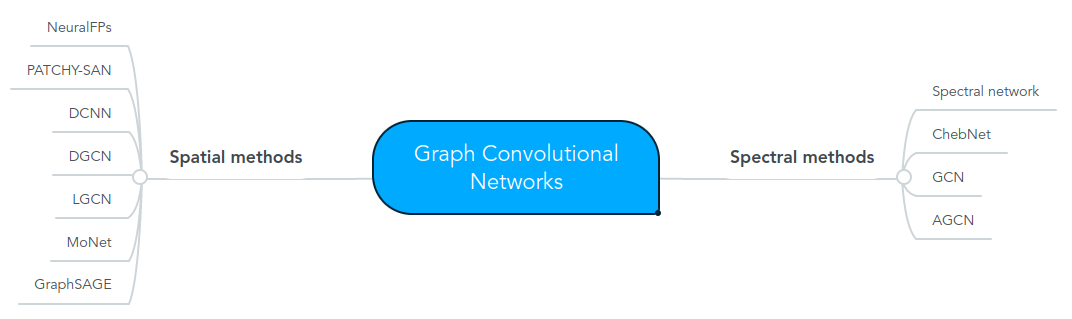
\includegraphics[width=1\linewidth]{figs/mindmap.png}
			\label{fig:writing-thesis}
		\end{figure}
	\end{frame}
	\begin{frame}{Problem statement}
		Similar to CNN, GCN is passing a filter over a graph, searching for important vertices and edges that can be used to classify nodes within the graph
		
		Problem statement: Given a graph $\mathcal{G} = \{\mathcal{V}, \mathcal{E}\}$, GCN
		\begin{itemize}
			\item Input: an input feature matrix $N \times F^{0}$ $\mathbf{X}$, where $N$ is the number of nodes, $ F^{0}$ is the number of input features; an $N \times N$ matrix representation of graph structure $\mathbf{A}$
			\item Output: feature of all neighbor nodes for each node, can be used for the next task like classification, link prediction, ...
		\end{itemize}
	\end{frame}
	\begin{frame}{Methodology}
		Consider a graph
		\begin{center}
			\begin{tikzpicture}[scale=0.5]
				[scale=.8,auto=left,every node/.style={circle,fill=blue!20}]
				\node (n6) at (1,10) {6};
				\node (n4) at (4,8)  {4};
				\node (n5) at (8,9)  {5};
				\node (n1) at (11,8) {1};
				\node (n2) at (9,6)  {2};
				\node (n3) at (5,5)  {3};
				\foreach \from/\to in {n6/n4,n4/n5,n5/n1,n1/n2,n2/n5,n2/n3,n3/n4}
				\draw (\from) -- (\to);
			\end{tikzpicture}
		\end{center}
		\begin{columns}
			\begin{column}{0.5\textwidth}
				\begin{gather*}
					\mathbf{A} = \begin{pmatrix}
						0 & 1 & 0 & 0 & 1 & 0\\
						1 & 0 & 1 & 0 & 1 & 0\\
						0 & 1 & 0 & 1 & 0 & 0\\
						0 & 0 & 1 & 0 & 1 & 1\\
						1 & 1 & 0 & 1 & 0 & 0\\
						0 & 0 & 0 & 1 & 0 & 0\\
					\end{pmatrix}
				\end{gather*}
			\end{column}
			\begin{column}{0.5\textwidth}
				\begin{gather*}
					\mathbf{X} = \begin{pmatrix}
						1 & -1\\
						2 & -2\\
						3 & -3\\
						4 & -4\\
						5 & -5\\
						6 & -6\\
					\end{pmatrix}
				\end{gather*}
			\end{column}
		\end{columns}
	\end{frame}
	\begin{frame}{Methodology}
		We can multiple $\mathbf{A}$ and $\mathbf{X}$ in order to obtain output
		\begin{gather*}
			\mathbf{A} \times \mathbf{X} = \begin{pmatrix}
				0 & 1 & 0 & 0 & 1 & 0\\
				1 & 0 & 1 & 0 & 1 & 0\\
				0 & 1 & 0 & 1 & 0 & 0\\
				0 & 0 & 1 & 0 & 1 & 1\\
				1 & 1 & 0 & 1 & 0 & 0\\
				0 & 0 & 0 & 1 & 0 & 0\\
			\end{pmatrix} \times \begin{pmatrix}
			1 & -1\\
			2 & -2\\
			3 & -3\\
			4 & -4\\
			5 & -5\\
			6 & -6\\
		\end{pmatrix} = \begin{pmatrix}
		7 & -7\\
		9 & -9\\
		6 & -6\\
		14 & -14\\
		7 & -7\\
		4 & -4\\
		\end{pmatrix}
		\end{gather*}
	\end{frame}
	\begin{frame}{Problem 1: Feature of the node itself}
	 	To addressing this problem, add an identity matrix $\mathbf{I}$ to  $\mathbf{A}$ before perform the multiplication
		\begin{gather*}
			\widetilde{\mathbf{A}} = \mathbf{A} + \mathbf{I}_n \\
			\begin{pmatrix}
				0 & 1 & 0 & 0 & 1 & 0\\
				1 & 0 & 1 & 0 & 1 & 0\\
				0 & 1 & 0 & 1 & 0 & 0\\
				0 & 0 & 1 & 0 & 1 & 1\\
				1 & 1 & 0 & 1 & 0 & 0\\
				0 & 0 & 0 & 1 & 0 & 0\\
			\end{pmatrix} + \begin{pmatrix}
			1 & 0 & 0 & 0 & 0 & 0\\
			0 & 1 & 0 & 0 & 0 & 0\\
			0 & 0 & 1 & 0 & 0 & 0\\
			0 & 0 & 0 & 1 & 0 & 0\\
			0 & 0 & 0 & 0 & 1 & 0\\
			0 & 0 & 0 & 0 & 0 & 1\\ 
		\end{pmatrix} = \begin{pmatrix}
		1 & 1 & 0 & 0 & 1 & 0\\
		1 & 1 & 1 & 0 & 1 & 0\\
		0 & 1 & 1 & 1 & 0 & 0\\
		0 & 0 & 1 & 1 & 1 & 1\\
		1 & 1 & 0 & 1 & 1 & 0\\
		0 & 0 & 0 & 1 & 0 & 1\\
	\end{pmatrix}
		\end{gather*}
	\begin{gather*}
		\widetilde{\mathbf{A}} \times \mathbf{X} = 
		\begin{pmatrix}
			1 & 1 & 0 & 0 & 1 & 0\\
			1 & 1 & 1 & 0 & 1 & 0\\
			0 & 1 & 1 & 1 & 0 & 0\\
			0 & 0 & 1 & 1 & 1 & 1\\
			1 & 1 & 0 & 1 & 1 & 0\\
			0 & 0 & 0 & 1 & 0 & 1\\
		\end{pmatrix} \times \begin{pmatrix}
		1 & -1\\
		2 & -2\\
		3 & -3\\
		4 & -4\\
		5 & -5\\
		6 & -6\\
	\end{pmatrix} = \begin{pmatrix}
	8 & -8\\
	11 & -11\\
	9 & -9\\
	18 & -18\\
	12 & -12\\
	10 & -10\\
	\end{pmatrix}
	\end{gather*}
	\end{frame}
	\begin{frame}{Problem 2: Normalization}
		To addressing this problem, we construct degree matrix $\mathbf{D}$ and use its inverse for multiplication
		\begin{columns}
			\begin{column}{0.5\textwidth}
				\begin{gather*}
					\mathbf{D} = \begin{pmatrix}
						2 & 0 & 0 & 0 & 0 & 0\\
						0 & 3 & 0 & 0 & 0 & 0\\
						0 & 0 & 2 & 0 & 0 & 0\\
						0 & 0 & 0 & 3 & 0 & 0\\
						0 & 0 & 0 & 0 & 3 & 0\\
						0 & 0 & 0 & 0 & 0 & 1\\ 
					\end{pmatrix}
				\end{gather*}
			\end{column}
			\begin{column}{0.5\textwidth}
				\begin{gather*}
					\mathbf{D}^{-1} = \begin{pmatrix}
						\frac{1}{2} & 0 & 0 & 0 & 0 & 0\\
						0 & \frac{1}{3} & 0 & 0 & 0 & 0\\
						0 & 0 & \frac{1}{2} & 0 & 0 & 0\\
						0 & 0 & 0 & \frac{1}{3} & 0 & 0\\
						0 & 0 & 0 & 0 & \frac{1}{3} & 0\\
						0 & 0 & 0 & 0 & 0 & 1\\ 
					\end{pmatrix}
				\end{gather*}
			\end{column}
		\end{columns}
		\begin{gather*}
			\mathbf{D}^{-1}\widetilde{\mathbf{A}}\mathbf{X} = \begin{pmatrix}
				\frac{1}{2} & 0 & 0 & 0 & 0 & 0\\
				0 & \frac{1}{3} & 0 & 0 & 0 & 0\\
				0 & 0 & \frac{1}{2} & 0 & 0 & 0\\
				0 & 0 & 0 & \frac{1}{3} & 0 & 0\\
				0 & 0 & 0 & 0 & \frac{1}{3} & 0\\
				0 & 0 & 0 & 0 & 0 & 1\\ 
			\end{pmatrix} \times \begin{pmatrix}
			8 & -8\\
			11 & -11\\
			9 & -9\\
			18 & -18\\
			12 & -12\\
			10 & -10\\
		\end{pmatrix} =  \begin{pmatrix}
		4 & -4\\
		11/3 & -11/3\\
		9/2 & 9/2\\
		6 & -6\\
		4 & -4\\
		10 & -10\\
		\end{pmatrix}
		\end{gather*}
	\end{frame}
	\begin{frame}{Apply weights}
		Consider a simple weight matrix $\mathbf{W} = \begin{pmatrix}1 \\ -1 \end{pmatrix}$
		\begin{gather*}
			\mathbf{D}^{-1}\widetilde{\mathbf{A}}\mathbf{X}\mathbf{W}
			= \begin{pmatrix}
				8 & -8\\
				11 & -11\\
				9 & -9\\
				18 & -18\\
				12 & -12\\
				10 & -10\\
			\end{pmatrix} \times \begin{pmatrix}1 \\ -1 \end{pmatrix}  = \begin{pmatrix}
			-8\\
			-22/3\\
			-9\\
			-12\\
			-8\\
			-20\\
		\end{pmatrix} 
		\end{gather*}
		Finally, like other neural networks, we can apply an activation function $\sigma$
		\begin{gather*}
			f(X, A) = \sigma(\mathbf{D}^{-1}\widetilde{\mathbf{A}}\mathbf{X}\mathbf{W})
		\end{gather*}
		In practice, we use a symmetric normalization $\mathbf{D}^{-1/2}\mathbf{A}\mathbf{D}^{-1/2}$
		\begin{gather*}
			f(X, A) = \sigma(\mathbf{D}^{-1/2}\widetilde{\mathbf{A}}\mathbf{D}^{-1/2}\mathbf{X}\mathbf{W})
		\end{gather*}
	\end{frame}
	\section{Variations of GCNs and its applications}
	\begin{frame}{Variations of GCNs}
		We have some variations of GCNs
		\begin{itemize}
			\item \textbf{Attention mechanisms}: capture the neighbor properties of the nodes, remember important nodes, give them higher weights
			\item \textbf{Graph Generative Networks}: similar to Generative Adversarial Network
			\item \textbf{Graph Spatial-Temporal Networks}: support the inputs that change over time
		\end{itemize}
		Application of GCNs
		\begin{itemize}
			\item Image Classification
			\item Community prediction
			\item Combinatorial Optimization
		\end{itemize}
	\end{frame}
	\section{Conclusion}
	\begin{frame}{Conclusion}
		For this presentation in this week, we introduced some basic about Graph Convolutional Networks
		\begin{itemize}
			\item An overview about Graph Convolutional Approach: \textbf{Spectral method} and \textbf{Spatial method}
			\item How Graph Convolutional Networks work?
			\item Some variations of GCNs
			\item Applications of GCNs
		\end{itemize}
	\end{frame}
	\begin{frame}{Q\&A}
		\huge Thanks for your attention with this presentation!
		
		\huge Any question? :)
	\end{frame}
	\begin{frame}{References}
		\nocite{*}
		\bibliography{references}\newpage\cleardoublepage
		\bibliographystyle{plain}
	\end{frame}
	
\end{document}